\documentclass[a4paper,11pt]{article}
%
% document setup, package import, etc.
%
%
% packages and settings for the worksheet files
%
\usepackage[bf,small]{titlesec}
\usepackage{graphicx}
\usepackage{amsfonts,amssymb,amsmath,fancyhdr}
%\usepackage{import} % needed for subimport
\usepackage{url}
\usepackage{paralist} % needed for compactenum
\usepackage{verbatim} % needed for varbatimiinput
\usepackage{shortlst}
\usepackage{siunitx}
%
%  page layout
%
\setlength{\textwidth}{175mm}
\setlength{\textheight}{240mm}
\setlength{\voffset}{-20mm}
\setlength{\hoffset}{-23mm}
\setlength{\parskip}{0pt}
\setlength{\parindent}{0pt}
\setlength{\footskip}{40pt}
\renewcommand{\baselinestretch}{1.2} \small\normalsize
%
%  Header/footer
%
\fancyhf{} % Clear all fields
\renewcommand{\headrulewidth}{0pt}
\renewcommand{\footrulewidth}{0pt}
\fancyfoot[L]{\footnotesize EMAT20920 2020-21}
\fancyfoot[C]{\footnotesize \thepage}
\fancyfoot[R]{\footnotesize COURSEWORK ASSESSMENT}
%
% Change list-making
%
\renewcommand{\theenumi}{\alph{enumi}}
\def\labelenumi{(\theenumi)}
\renewcommand{\theenumii}{\roman{enumii}}
\def\labelenumii{(\theenumii)}
%
% Change section headers
%
\titlelabel{Question \thetitle:\quad}
%
% First page header
%
\newcommand{\solutionsheader}[2]{
    \pagestyle{fancy}
    \begin{center}
      {\large Department of Engineering Mathematics}\\[3ex]
      \textbf{EMAT20920: Numerical Methods in MATLAB}\\[3ex]
      \textbf{#1}\\
      \textbf{#2}
    \end{center}}
%
% For formatting matlab code with listings
%
\usepackage{listings}
\usepackage{color}
\usepackage{textcomp}
\definecolor{listinggray}{gray}{0.9}
\definecolor{lbcolor}{rgb}{0.9,0.9,0.9}
\lstset{
    backgroundcolor=\color{lbcolor},
    numbers=none,
    numberstyle=\tiny,
    tabsize=4,
    rulecolor=,
    language=matlab,
    basicstyle=\scriptsize\ttfamily,
    upquote=true,
    aboveskip={1.5\baselineskip},
    columns=flexible,
    showstringspaces=false,
    extendedchars=true,
    breaklines=true,
    prebreak = \raisebox{0ex}[0ex][0ex]{\ensuremath{\hookleftarrow}},
    %frame=single,
    showtabs=false,
    showspaces=false,
    showstringspaces=false,
    identifierstyle=\ttfamily,
    keywordstyle=\color[rgb]{0,0,1},
    commentstyle=\color[rgb]{0.133,0.545,0.133},
    stringstyle=\color[rgb]{0.627,0.126,0.941},
    aboveskip=0pt,
    belowskip=2pt,
}
%
% shortcut commands
%
\newcommand{\matcmd}[1]{\colorbox{lbcolor}{\lstinline{#1}}}
\newcommand{\matlab}[1]{\texttt{#1}}
\renewcommand{\vec}[1]{\boldsymbol{#1}}
\newcommand{\order}{\mathcal{O}}

\begin{document}

\solutionsheader{WORKSHEET 6 --- SOLUTIONS}{NUMERICAL SOLUTION OF ODEs}


\section{Forward and Backward Euler}

\begin{enumerate}
  \item Timesteps $h=0.5$, $h=0.1$ and $h=0.01$ correspond to $N=2$, $N=10$ and $N=100$ respectively.
    Calling \matlab{myEuler} with values as in the question 
\begin{lstlisting}
[t2,y2]=myEuler(@(t,y) t-10*y,[0 1],1,2);
[t10,y10]=myEuler(@(t,y) t-10*y,[0 1],1,10);
[t100,y100]=myEuler(@(t,y) t-10*y,[0 1],1,100);
\end{lstlisting}
    and plotting the results together with the exact solution leads to the following three graphs:
    \begin{center}
      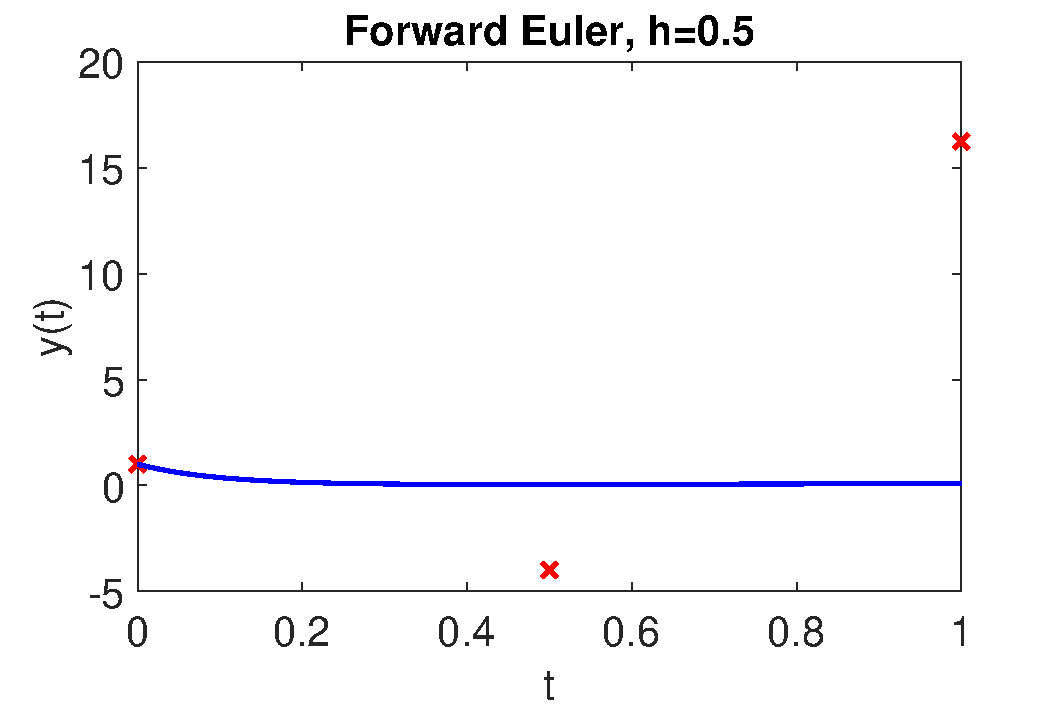
\includegraphics[scale=0.3]{images/Q1a_1.pdf}
      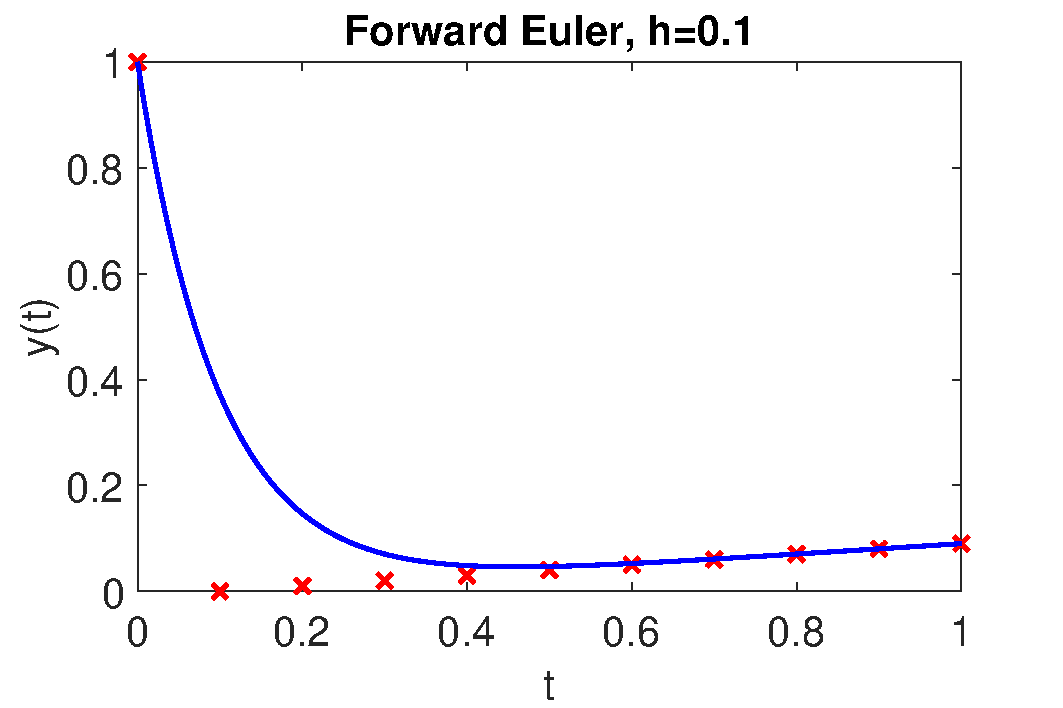
\includegraphics[scale=0.3]{images/Q1a_2.pdf}
      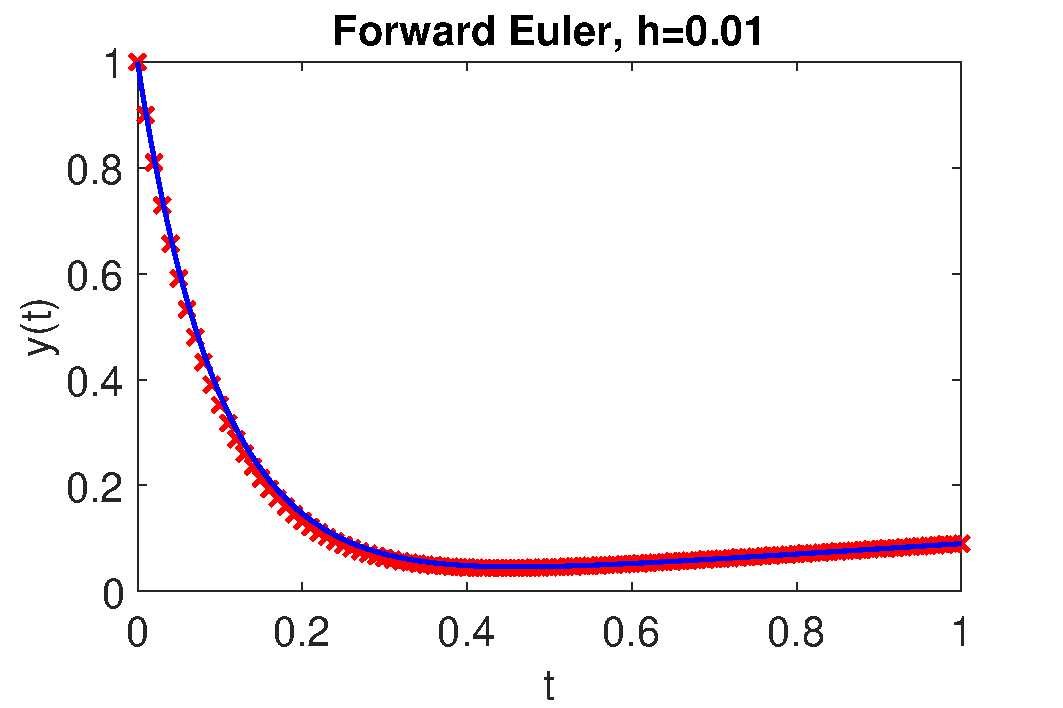
\includegraphics[scale=0.3]{images/Q1a_3.pdf}
    \end{center}
    Only the last, with timestep $h=0.01$, gets the solution right for all $t=[0,5]$.
    The first, with timestep $h=0.5$ is qualitatively (and badly) wrong --- it oscillates and grows (note the very different scale on the
    vertical axis). This is caused by the (conditional) instability of the forward Euler
    method.
    
    We see the same effects, more dramatically, by solving up to $t=5$ instead of $t=1$ (using $N=10$, $N=50$ and $N=500$, to get the same stepsizes $h=0.5$, $h=0.1$ and $h=0.01$ respectively), yielding the following graphs:
    \begin{center}
      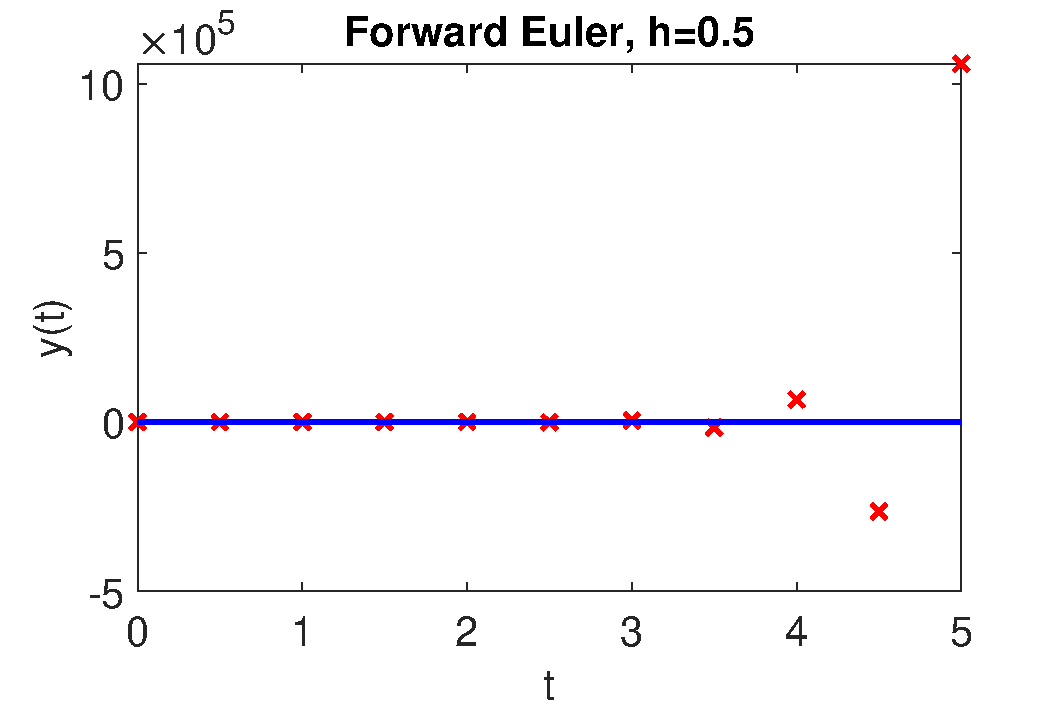
\includegraphics[scale=0.3]{images/Q1a_4.pdf}
      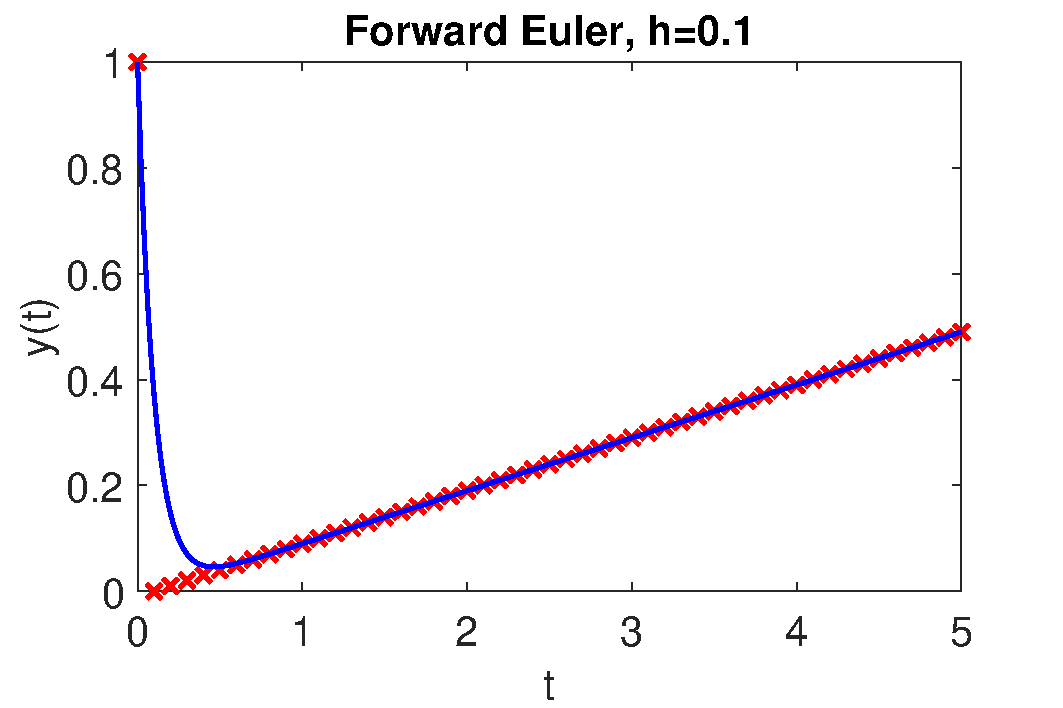
\includegraphics[scale=0.3]{images/Q1a_5.pdf}
      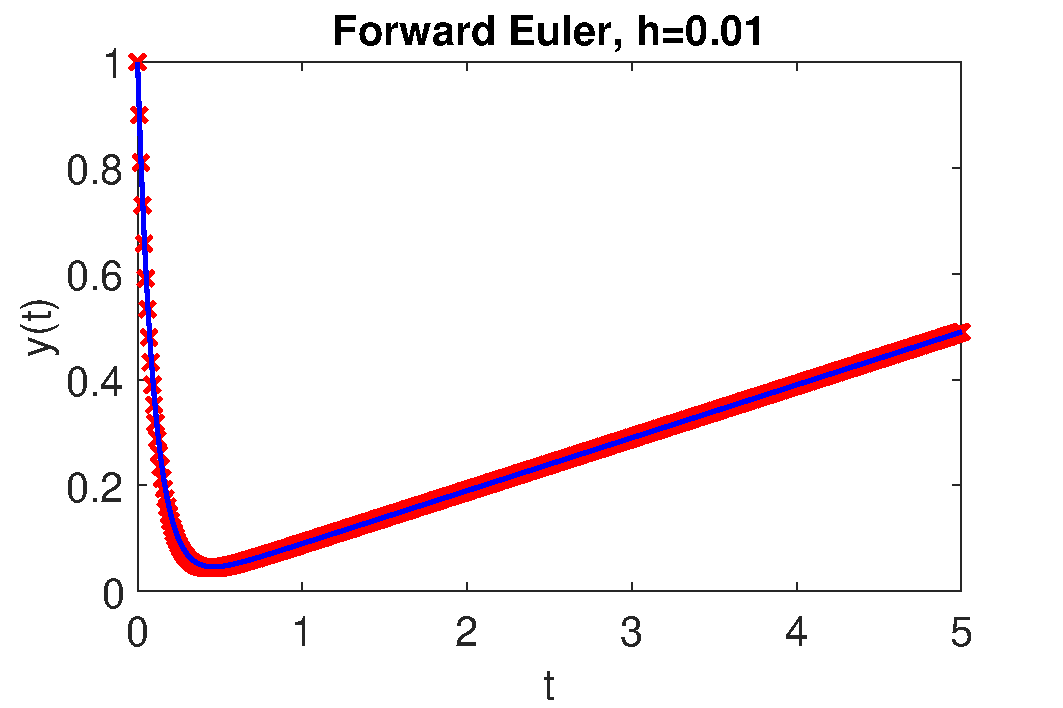
\includegraphics[scale=0.3]{images/Q1a_6.pdf}
    \end{center}
    
    
    \begin{enumerate}
    

      \item The right-hand-side function in this case is $f(t,y)=t-10y$. Using this in the
    backward Euler iteration we get
    \begin{align*}
      y_{k+1} &= y_k + hf(t_{k+1},y_{k+1}) \\
        &= y_k + h(t_{k+1} - 10y_{k+1}) \\
        &= y_k + ht_{k+1} - 10hy_{k+1}\\
      (1+10h)y_{k+1} &= y_k +ht_{k+1} \\
      y_{k+1} &= \frac{y_k+ht_{k+1}}{1+10h}\\
        &= \frac{y_k+h(t_k+h)}{1+10h} \qquad\text{(using $t_{k+1}=t_k+h$)}
    \end{align*}
    A simple MATLAB code to execute this is the following:
    \lstinputlisting{scripts/backwardEuler.m}
    which gives the following results for $t\in[0,1]$:
    \begin{center}
      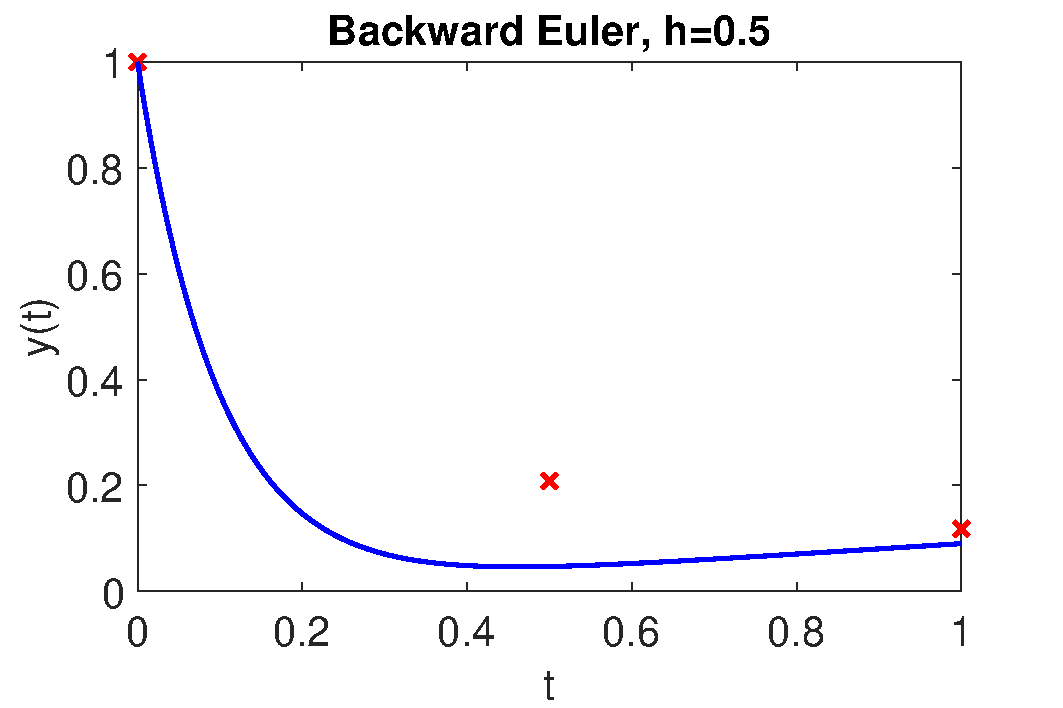
\includegraphics[width=0.3\linewidth]{images/Q1b_1.pdf}
      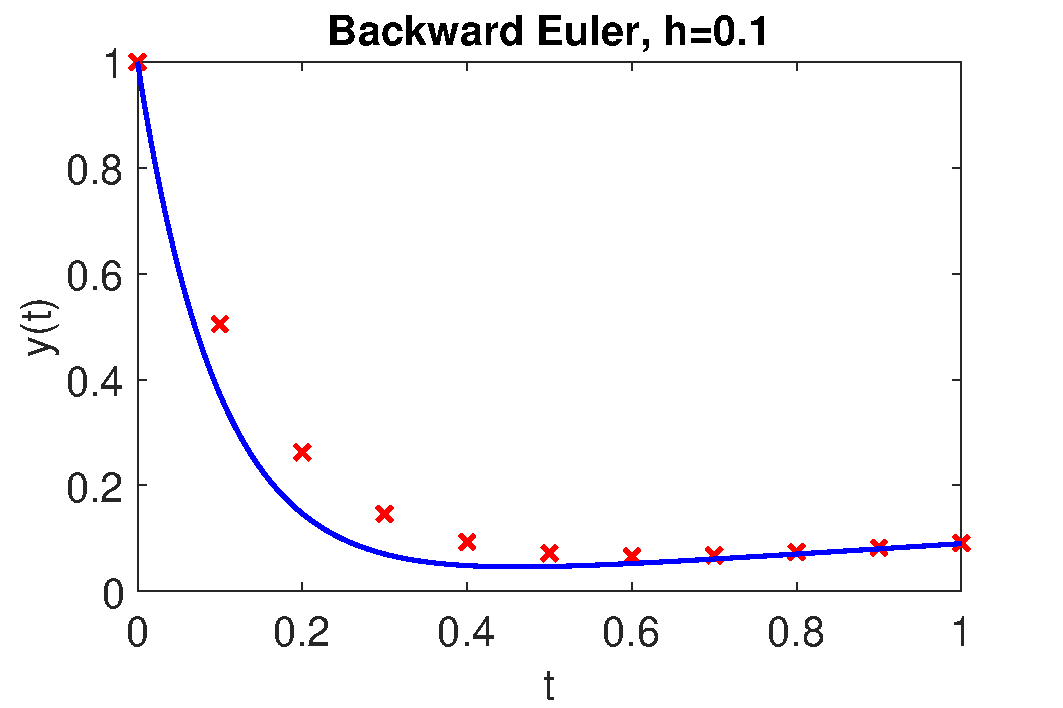
\includegraphics[width=0.3\linewidth]{images/Q1b_2.pdf}
      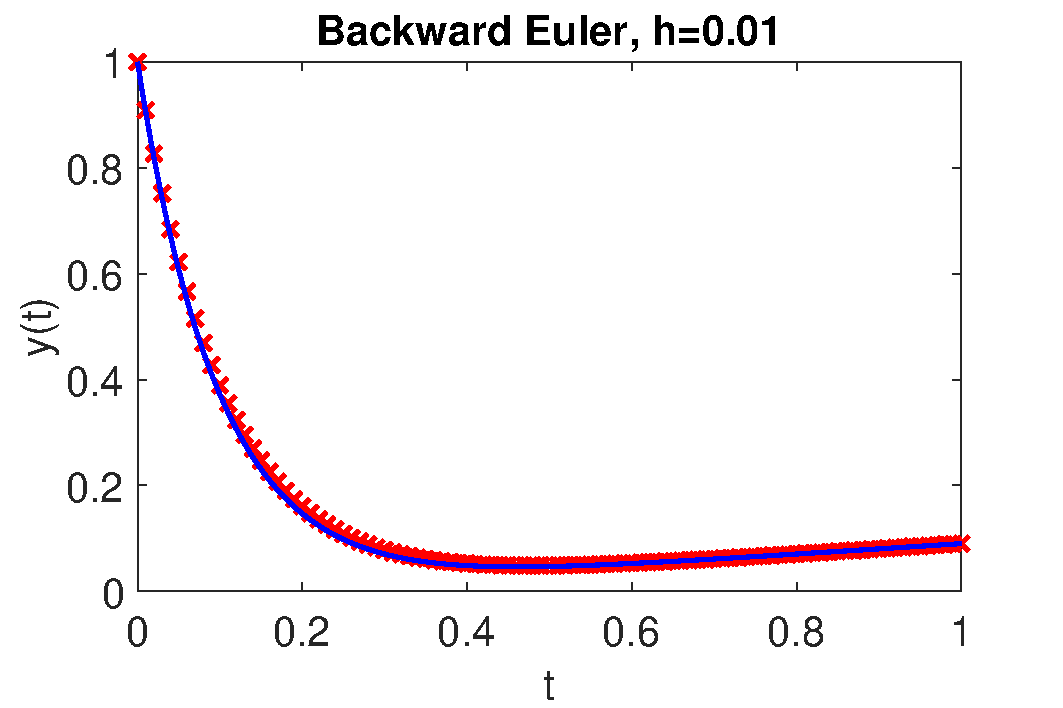
\includegraphics[width=0.3\linewidth]{images/Q1b_3.pdf}
    \end{center}
    and for  $t\in[0,5]$:
    \begin{center}
      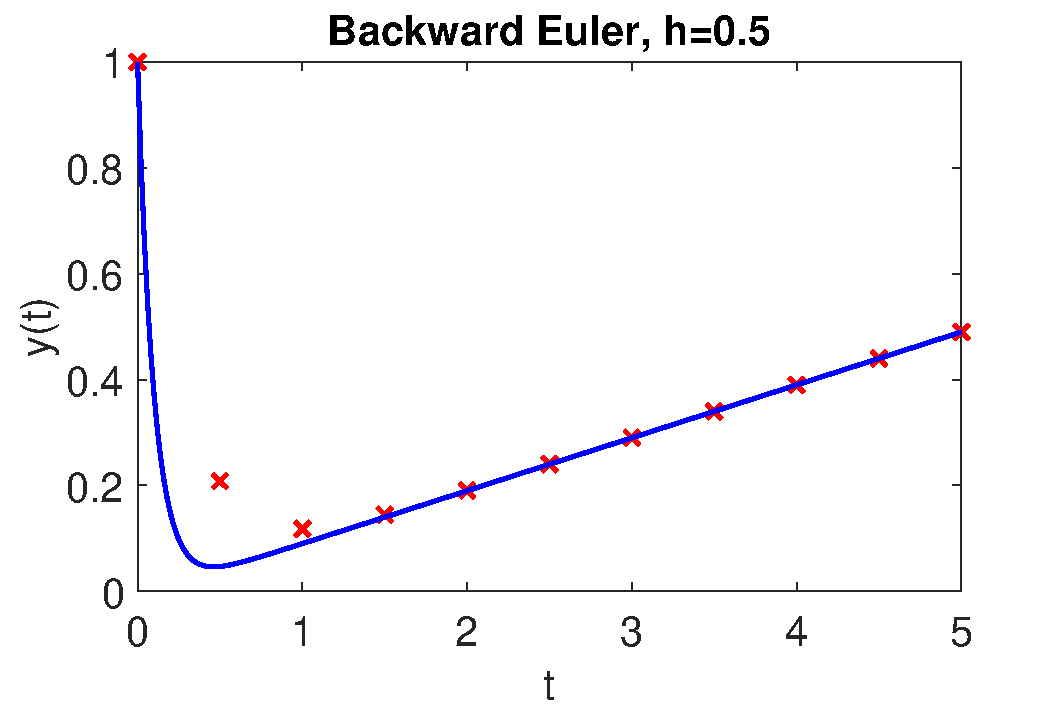
\includegraphics[width=0.3\linewidth]{images/Q1b_4.pdf}
      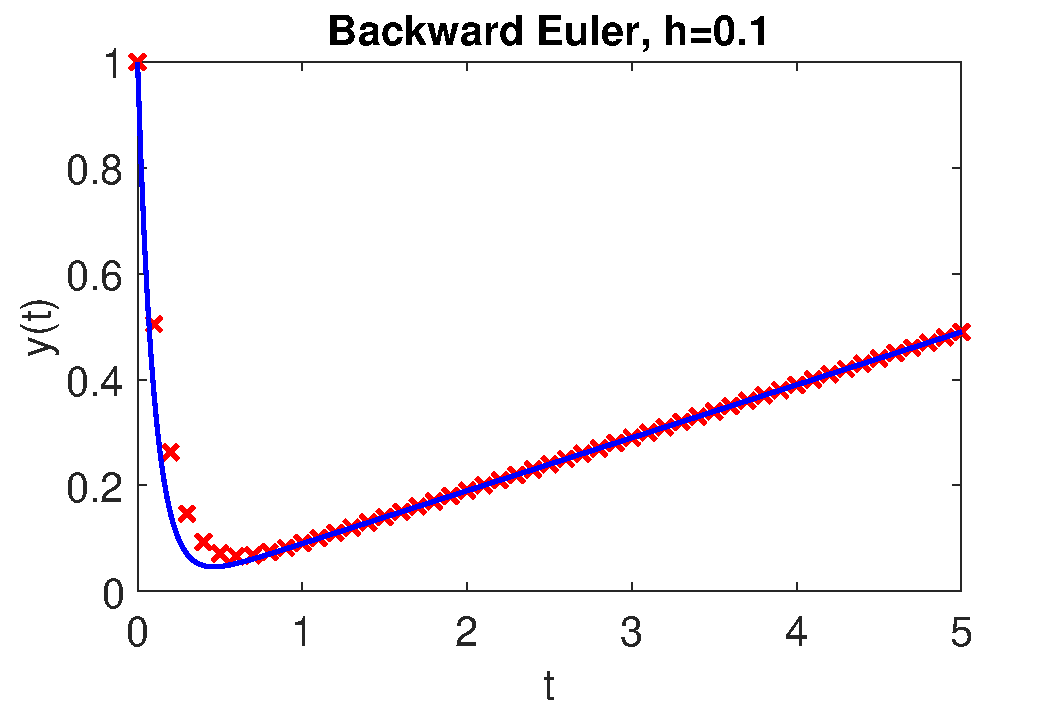
\includegraphics[width=0.3\linewidth]{images/Q1b_5.pdf}
      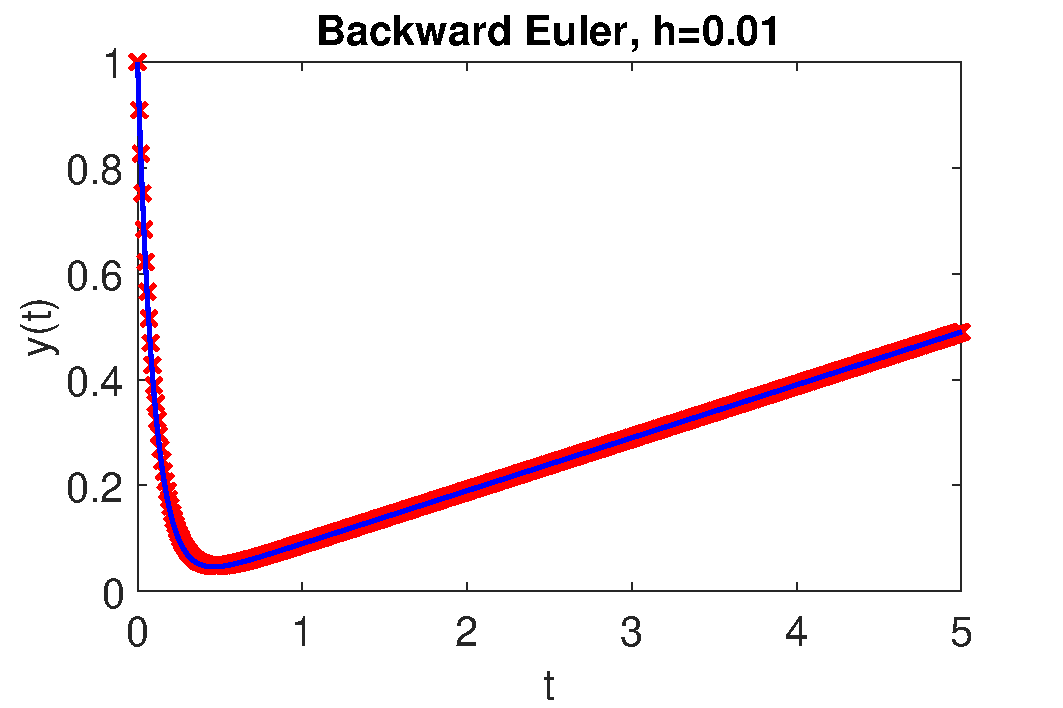
\includegraphics[width=0.3\linewidth]{images/Q1b_6.pdf}
    \end{center}
    
    Now all  results are qualitatively correct, with improving accuracy as $h\rightarrow0$,
    as the Backward Euler method is unconditionally stable. Unfortunately, though, it's not
    often possible to (re)write the iteration in an explicit way; we have been lucky with the
    function $f$ here.
    
  \item The following MATLAB script will find the absolute error between numerical and
    exact solution at $t=1$, and plot a graph:
    \lstinputlisting{scripts/backwardEulererror.m}
    Note the use of \matlab{floor} in the code above, which rounds numbers down to the nearest integer: the number of timesteps $N$ must be an integer.
    
    The resulting error vs. timestep plot is:
    \begin{center}
      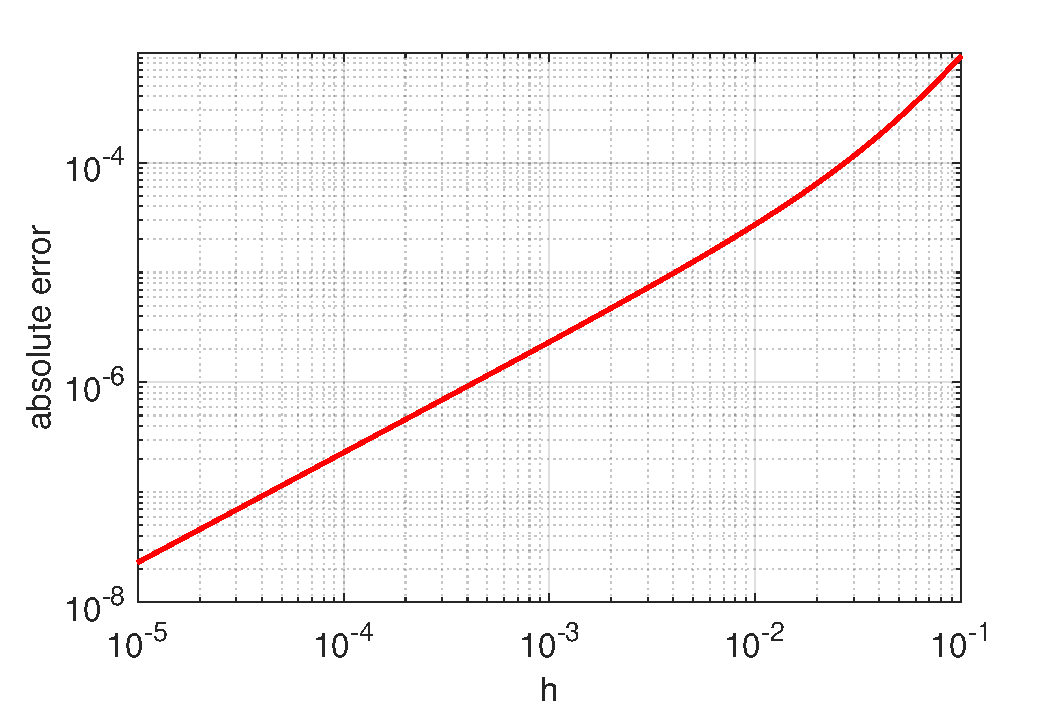
\includegraphics[width=0.75\linewidth]{images/Q1bii.pdf}
    \end{center}
    
    Reading off the graph, the gradient is equal to $1$ (in the straight line portion of the graph --- remember that, strictly speaking, we have to take the limit $h\rightarrow0$), and so the backward Euler method has global truncation error of $\order(h)$, as expected.
   \end{enumerate}
   
   \item
   
   \begin{enumerate}
   
     \item The trapezoid method, from the lecture notes, is given by
       \begin{equation*}
         y_{k+1}=y_k+\frac{h}{2} \Bigl[ f(t_k,y_k)+f(t_{k+1},y_{k+1}) \Bigr]
       \end{equation*}
       Again we can plug in the right-hand-side function    $f(t,y)=t-10y$, and rearrange to find $y_{k+1}$ in terms of $y_k$:       
    \begin{align*}
      y_{k+1} &= y_k + \frac{h}{2}\Bigl[ f(t_k,y_k)+f(t_{k+1},y_{k+1}) \Bigr] \\
        &= y_k + \frac{h}{2}\Bigl[ t_k-10y_k + t_{k+1}-10y_{k+1} \Bigr]\\
        &= y_k + \frac{h}{2}(t_k+t_{k+1}) -5hy_k -5hy_{k+1}\\
        (1+5h)y_{k+1} &= (1-5h)y_k + \frac{h}{2}(t_k+t_{k+1})\\
        y_{k+1} &= \left(\frac{1-5h}{1+5h}\right)y_k + \frac{h(t_k+t_{k+1})}{2(1+5h)}\\
        &= \left(\frac{1-5h}{1+5h}\right)y_k + \frac{h(t_k+h/2)}{1+5h} \qquad\text{(using $t_{k+1}=t_k+h$)}
    \end{align*}
    The following code will implement this iteration to solve the ODE:
    \lstinputlisting{scripts/trapezoid.m}
    from which we can obtain the following results for $y(t)$, over the intervals $[0,1]$ and $[0,5]$:
    \begin{center}
      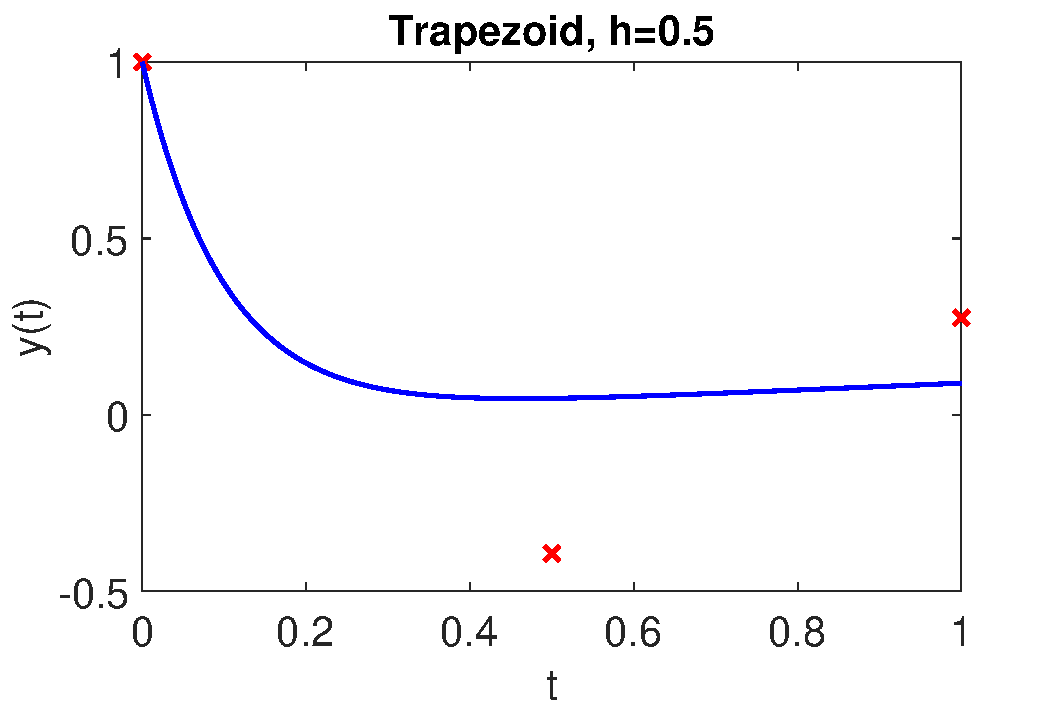
\includegraphics[width=0.3\linewidth]{images/Q1c_1.pdf}
      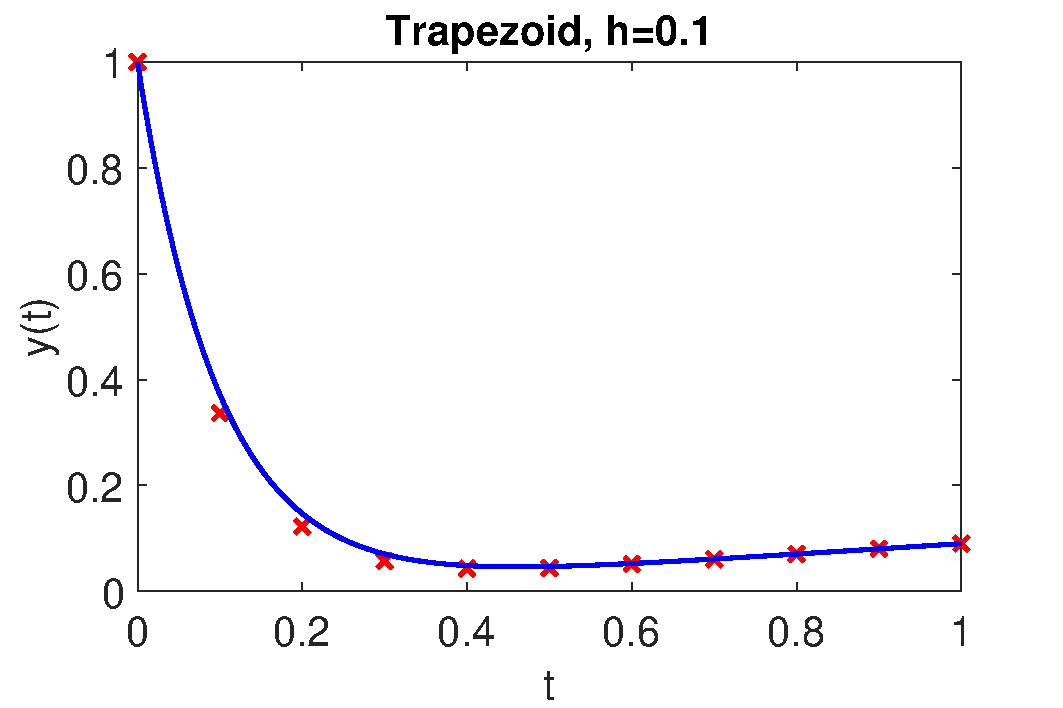
\includegraphics[width=0.3\linewidth]{images/Q1c_2.pdf}
      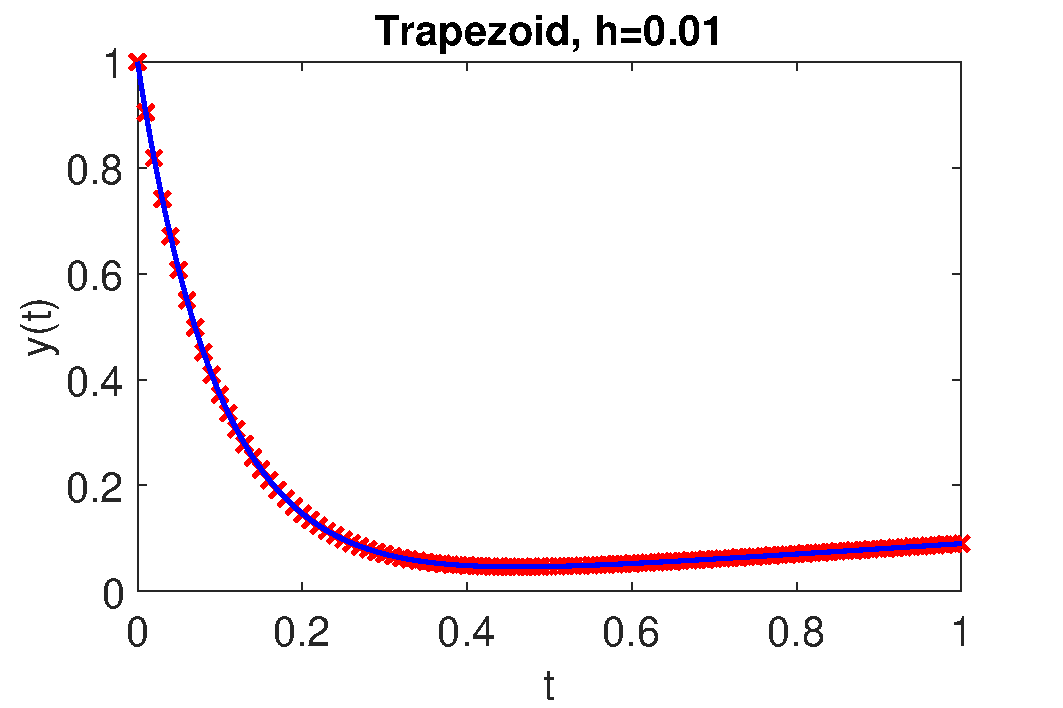
\includegraphics[width=0.3\linewidth]{images/Q1c_3.pdf}\\
%    \end{center}
%    \begin{center}
      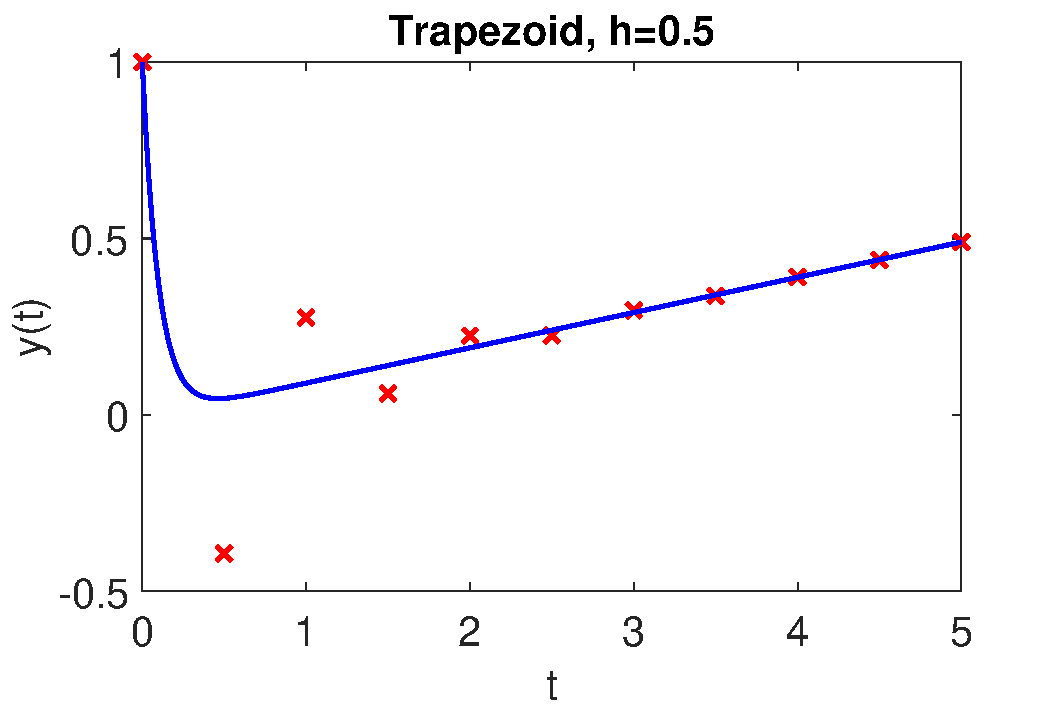
\includegraphics[width=0.3\linewidth]{images/Q1c_4.pdf}
      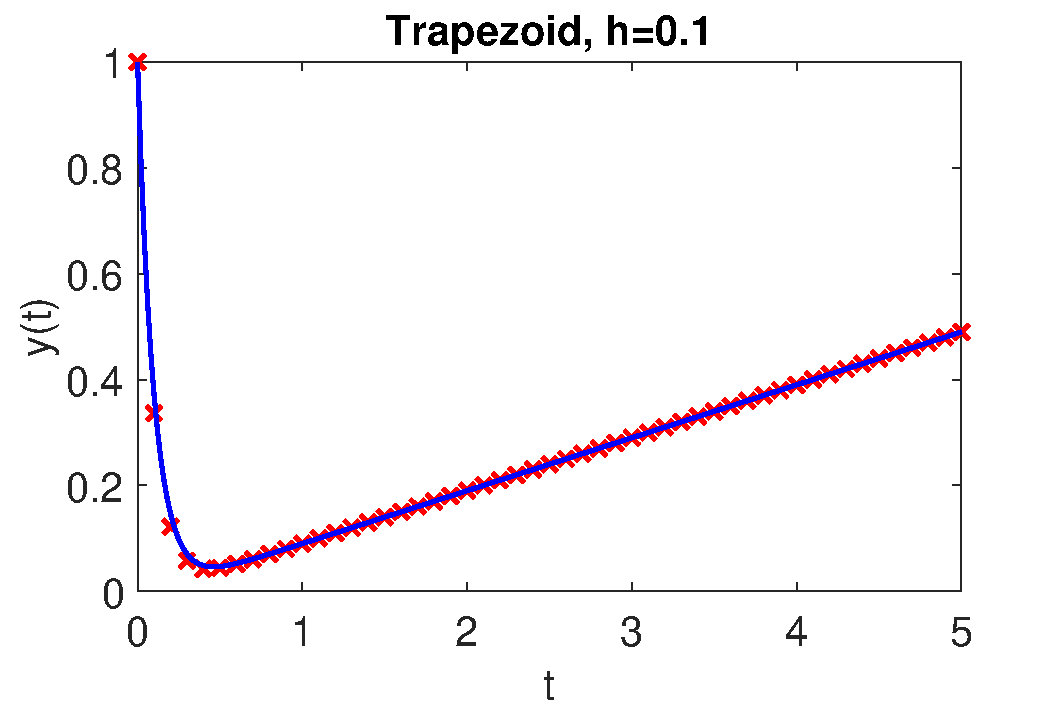
\includegraphics[width=0.3\linewidth]{images/Q1c_5.pdf}
      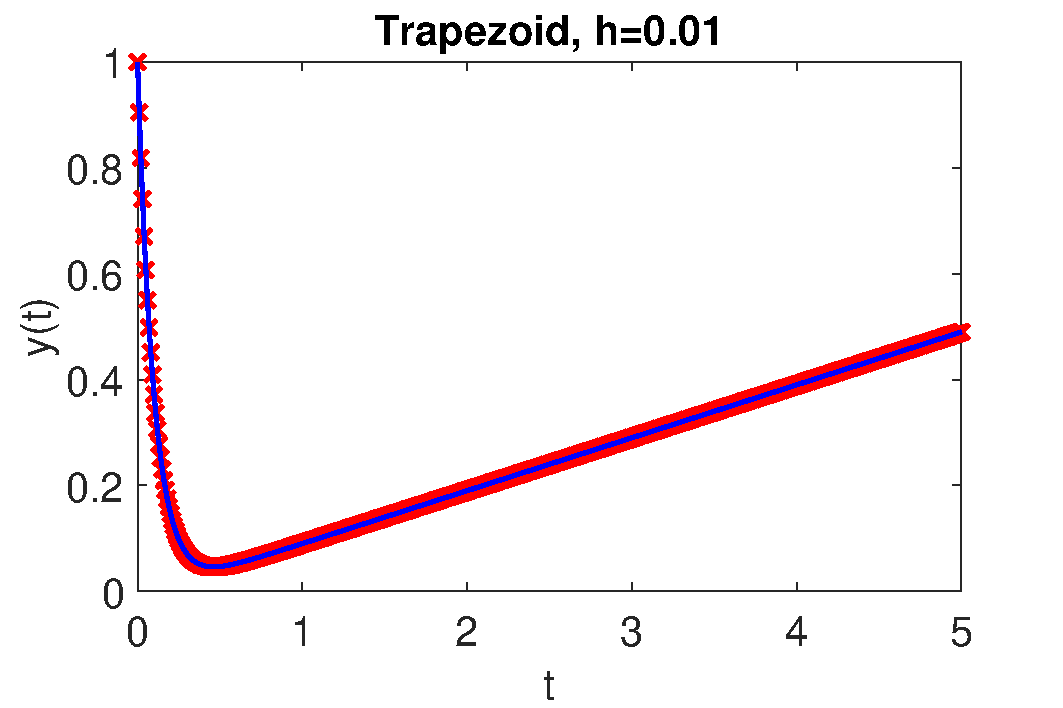
\includegraphics[width=0.3\linewidth]{images/Q1c_6.pdf}
    \end{center}
    We see that the trapezoid method is unconditionally stable. There's a hint of instability about the left-hand images, $h=0.5$, but the iteration recovers to provide the right qualitative behaviour; decaying transient oscillation can still take place in unconditionally stable methods.
    
    We can find the global truncation error in exactly the same way as before:
    \lstinputlisting{scripts/trapezoiderror.m}
    which gives the error versus stepsize result
    \begin{center}
      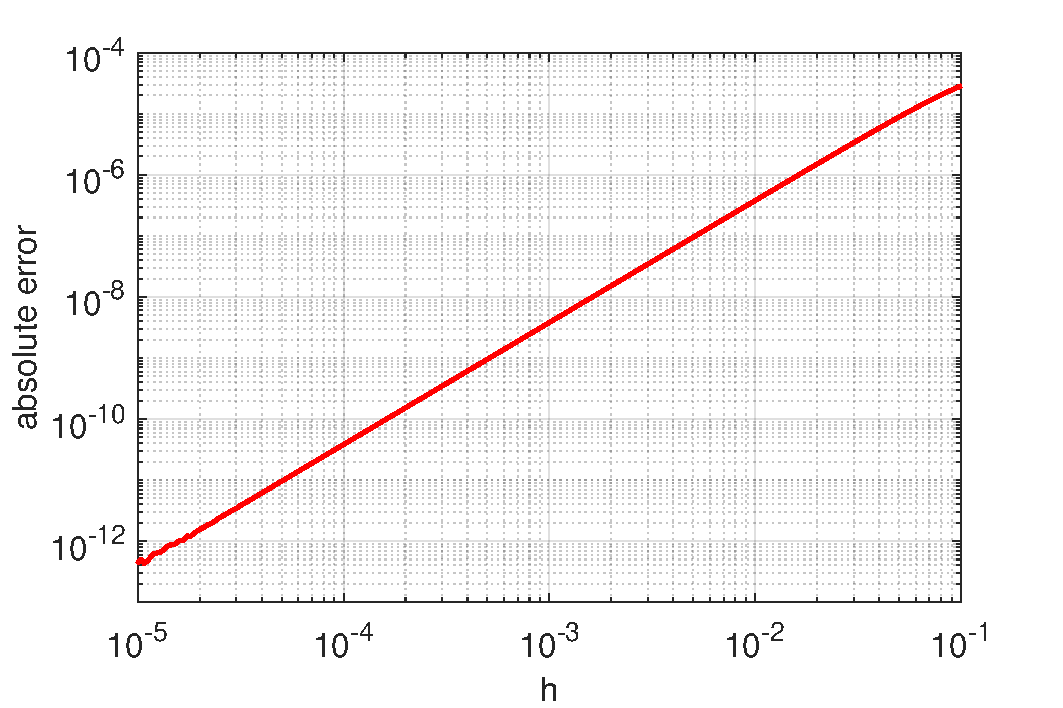
\includegraphics[width=0.75\linewidth]{images/Q1cii.pdf}
    \end{center}
    from which we can conclude that the slope of the graph is 2, and hence that the global truncation error of the trapezoid method is $\order(h^2)$; i.e., it's a second order scheme.
    
   
   \end{enumerate}

    \end{enumerate}


\section{Event detection in \matlab{ode45}}

\begin{enumerate}

\item
\begin{enumerate}
  \item We write $y_1=x$, $y_2=\dot{x}$ to transform the 2nd order ODE into a system of two 1st order
    ODEs (for $\vec{y}=(y_1,y_2)^T$). In MATLAB this can be written as follows:
    \lstinputlisting{scripts/rhs_spring_v1.m}
    
    It's not the best way to write the function, though; it would be preferable to pass the parameters as inputs, particularly as later one of them ($m$) will vary during the simulation. We'll come back to this idea in part (b).
    
  \item We can solve the ODE, and plot graphs of position $x$ and velocity $\dot{x}$ versus time $t$, by typing:
\begin{lstlisting}
[t,y]=ode45(@rhs_spring_v1,[0 5],[0.1;-0.05]);
subplot(2,1,1);
plot(t,y(:,1),'r-');
xlabel('t'); ylabel('x');
xlim([0 5]);
subplot(2,1,2);
plot(t,y(:,2),'r-');
xlabel('t'); ylabel('dx/dt');
xlim([0 5]);
\end{lstlisting}

The results look as follows:
\begin{center}
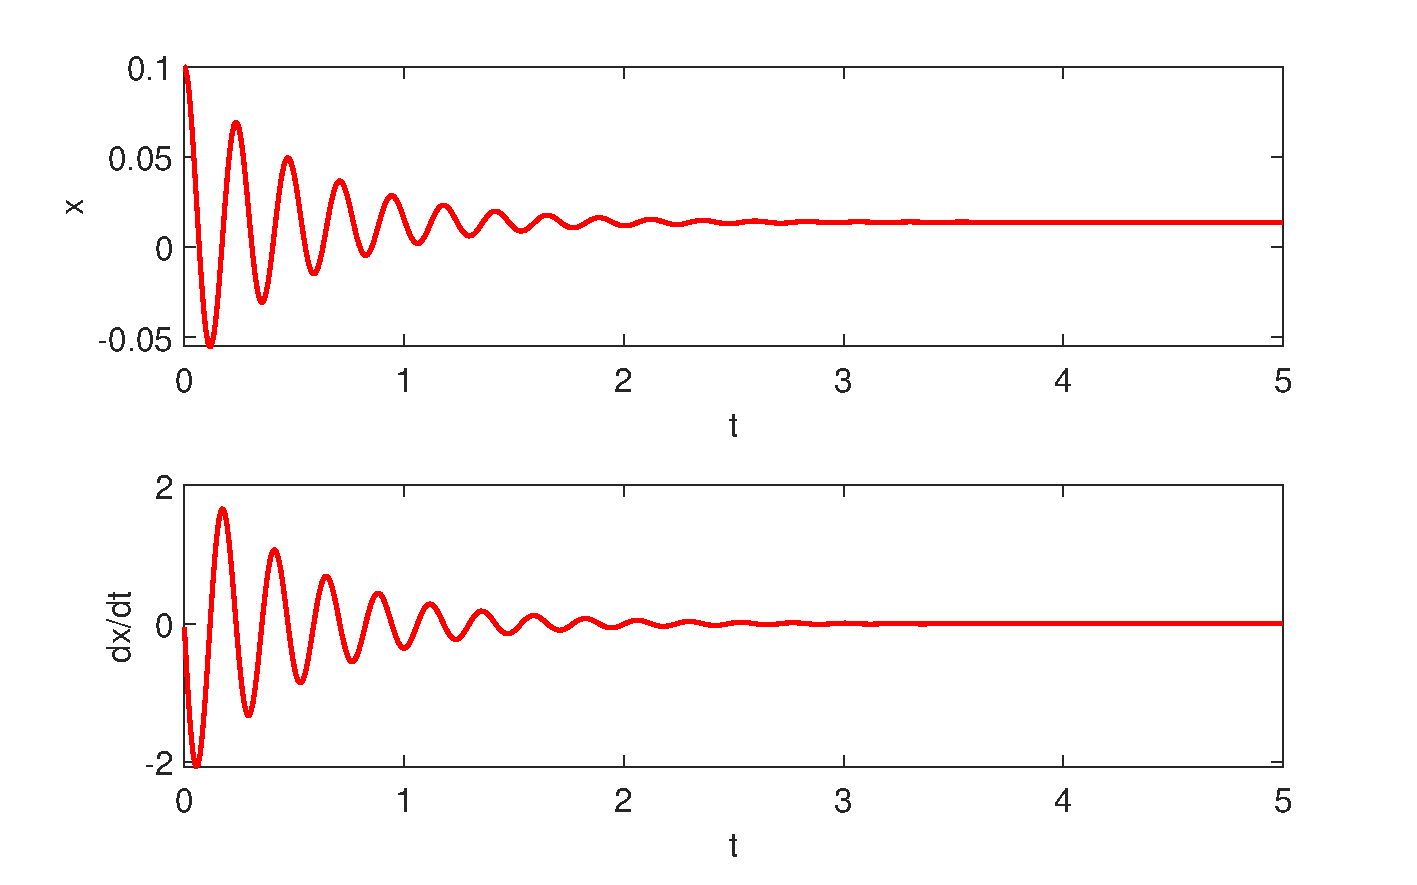
\includegraphics[width=0.9\linewidth]{images/Q2a.pdf}
\end{center}
The mass oscillates, with constant frequency, and settles to a steady displacement of around $x=0.01$, with zero velocity. The mass-spring-damper system is underdamped.
    
\end{enumerate}

\item
\begin{enumerate}

  \item In this part, we're going to have to deal with a non-constant mass, so we need to update the ODE right-hand-side function to have the mass as an input: 
    \lstinputlisting{scripts/rhs_spring_v2.m}

    Turning to the events function, to detect a maximum of $x(t)$ we need to look for zeros of velocity, $\dot{x}=y_2$, crossing zero from positive to negative velocity (i.e., decreasing). We'll also need to stop the integration so we can change the mass. That's all achieved by the following events function:
    \lstinputlisting{scripts/springEvent.m}
    
  \item The following MATLAB script can be used to run the simulation, and plot graphs of
    position and velocity versus time, as required.
    \lstinputlisting{scripts/runspring.m}
%    The events function, used to detect the first maximum of $y$, i.e.\ the first zero of $\dot{y}=x_2$
%    (\matlab{val=x(2)}) with $\dot{y}$ going from positive to negative (\matlab{dir=-1}), and stop the
%    integration (\matlab{term=1}), is as follows:
    
    The results are as follows (the time \matlab{te} when the mass is added is marked with a dotted line and a cross at the position \matlab{ye(1)} and velocity {ye(2)}):
    \begin{center}
      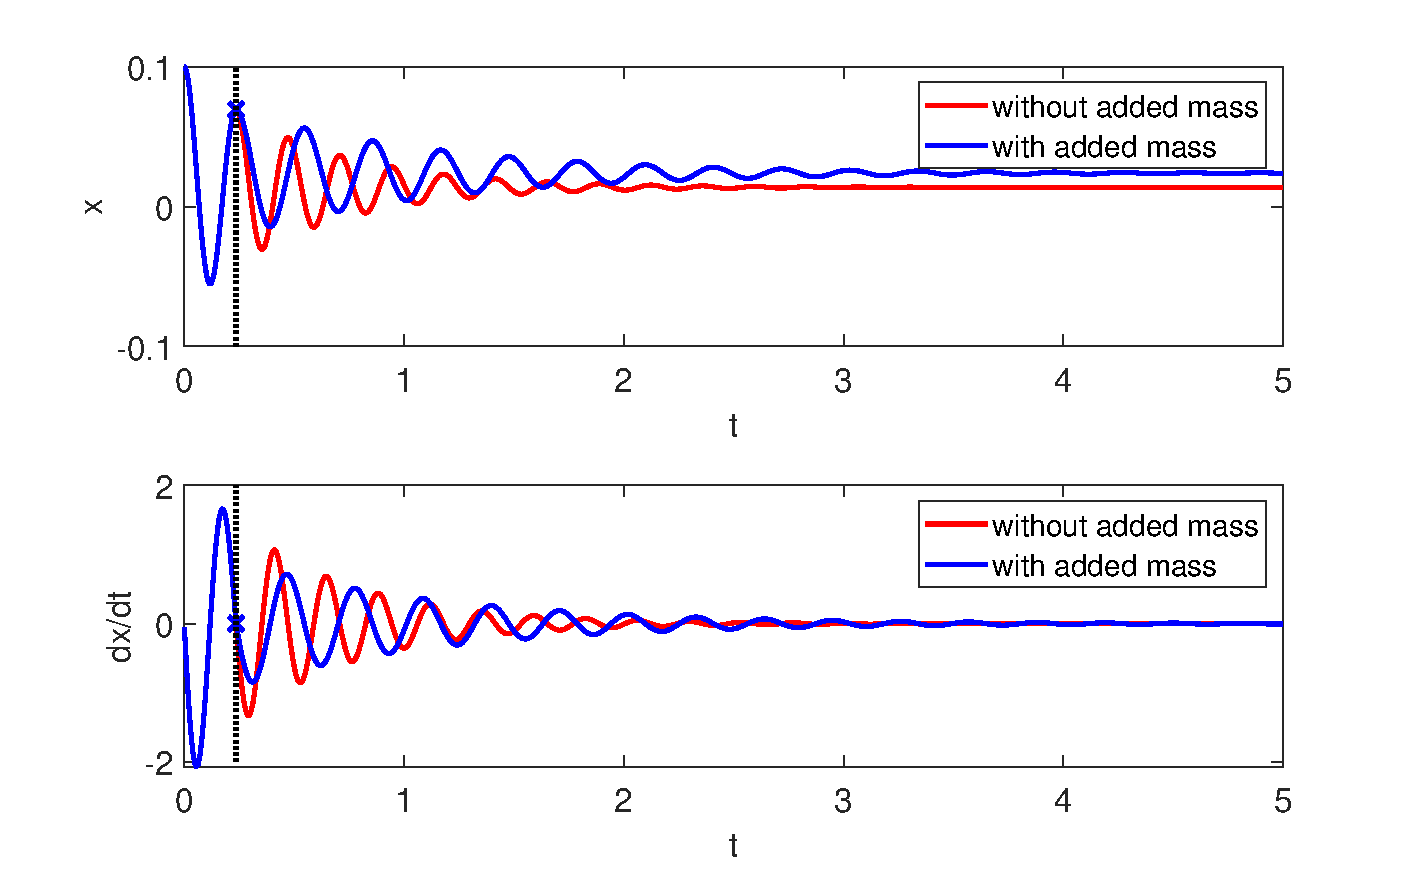
\includegraphics[width=0.9\linewidth]{images/Q2b}
    \end{center}

  \item The simulation shows that adding the mass causes a change in the equilibrium position (the
    mass comes to rest at a larger value of $x$, i.e.\ lower down), and also in the frequency of
    motion (more rapid oscillations). The latter effect is perhaps more clearly seen in the
    velocity versus time graph. The mass-added system takes longer to come to rest, too.
\end{enumerate}

\end{enumerate}


\end{document}
